\documentclass[../main.tex]{subfiles}

\begin{document}
\section{Introduction: the spectrum and its approximation}
The computation of spectra can boldly be considered the 'fundamental problem of operator theory' \parencite{arveson2002short}. The spectrum
of an operator holds the same key to the entire structure as eigenvalues do for linear algebra, however (as often occurs when passing from 
the finite- to infinite-dimensional case) we lose the ease of representation that allows the creation of such algorithms and formulae as those 
used for matrices. 

\subsection{Spectra}

We must first define our quantity of interest: the spectrum of an operator.
\begin{definition}{\textbf{(Resolvent and spectrum)}}\index{resolvent}\index{spectrum}
(Adapted from \parencite{edmunds2018spectral}) Let $T$ be a linear operator on a Banach space.
\begin{itemize}
\item The resolvent of $T$ is the set $\rho(T) := \{\eta \in \mathbb{C} : (T - \eta I)\text{ has a bounded inverse}\}$, where I is the identity operator. 
If it exists, we call its inverse $(T - \eta I)^{-1}$ the `resolvent operator' for $\eta$ and $T$.
\item The spectrum of $T$, denoted $\Spec(T)$, is $\mathbb{C} \setminus \rho(T)$, i.e. the set of all complex numbers $\lambda$ such 
that the operator $(T - \lambda I)$ does not have a bounded inverse.
\end{itemize}
\end{definition}

In the remainder of the text, the identity operator $I$ will be implicit in the operator - i.e. we will simply write $(T - \lambda I)$ as $(T - \lambda)$.

One can see that this concept generalises the eigenvalues of a matrix to any Banach space, and that for a finite-dimensional Banach space
(of which $\mathbb{R}^n$ and $\mathbb{C}^n$ are major examples) we can recover the eigenvector equation. Indeed, the term `resolvent'
originates from its relation to the solution of certain types of differential equation; if for some differential operator $L$ we have the equation
$Lu = \lambda u + g$, a solution $u$ would be related to $g$ as $(L - \lambda)^{-1}g = u$. 

For an operator on an
infinite-dimensional space, values which satisfy the eigenvector equation \emph{are} in the spectrum of the operator, but they do not
comprise the entire spectrum - nor do we necessarily have a spectrum made up of a discrete set of values.

\begin{example}
Let $S$ be the 'right-shift' operator on the sequence space $\ell^2(\mathbb{N})$, which has the following action:
$S(x_1, x_2, x_3, ...)$ = $(0, x_1, x_2, x_3, ...)$; that is, for a sequence $u$ we map $u_n$ to $u_{n+1}$, and pad the vector with a zero in $u_1$'s place.
$S$ has no eigenvalues, and its spectrum is the open unit disc $D = \{z \in \mathbb{C} : |z| = 1\}$.
\end{example}
\begin{proof}{\emph{(sketch)}}
For the lack of eigenvalues; we see that if $Su = \lambda u$, 
$$(0, u_1, u_2, u_3 ...) = (\lambda u_1, \lambda u_2, \lambda u_3 ...)$$
so in particular, we would require $\lambda u_1 = 0$. Then either $\lambda = 0$ and thus $u_n$ = 0 for all $n$, or as $\lambda \neq 0$, $u_1 =0$. Then $\lambda u_2 = u_1 = 0$, and continuing this we
can see that $u_n = 0$ for all $n$, i.e. $u$ must be the zero vector. Thus there is no non-zero vector satisfying the eigenvector equation.

To calculate its spectrum, we make use of a natural relation between the spectrum of an operator T and the spectrum of its adjoint: 
\begin{align*}
\lambda \in \Spec(T)  &\text{ iff } (T - \lambda)\text{ is not invertible }\\
& \text{ iff } (T - \lambda)^*\text{ is not invertible (this is true for any operator)}\\
& = (T^* - \overline{\lambda}) \text{ not invertible, i.e. } \overline{\lambda} \in \Spec(T^*).
\end{align*}
in this case, the adjoint is the left-shift operator $S^*u = (u_2, u_3, u_4, ...).$; we can see that for any value $\lambda$ we have for the vector
$(\lambda, \lambda^2, \lambda^3...)$
$$S^*(\lambda, \lambda^2, \lambda^3) = (\lambda^2, \lambda^3, \lambda^4, ...) = \lambda(\lambda, \lambda^2, \lambda^3...)$$
which is in $\ell^2(\mathbb{N})$ and is thus an eigenvector iff $|\lambda| < 1$; hence the unit disc is in $\Spec(S^*)$ and hence its
complex conjugate (which is also the unit disc) is in $\Spec(S)$.
\end{proof}

As we have alluded to, there is no universal algorithm for the calculation of operator spectra in the way that there is the QR algorithm \cite{suli2003introduction} for matrices. To devise a formula for the spectrum of even a specific subset of a class of operators is a mathematical
feat, and varieties of operators important to fields such as quantum physics (\cite{lewin2010spectral}), hydrodynamics (\cite{manning2008descriptor}), and crystallography (\cite{cances2012periodic}) still withhold the structure of their spectra from decades-long attempts at discovery. 
To this end, we must employ numerical methods.
We shall find that even approximating spectra computationally is not so easy.

\subsection{Approximating spectra; Ritz-Galerkin methods}

It would be a reasonable hypothesis that we can approximate spectra by reducing the infinite-dimensional problem to a finite-dimensional one, where
we are on much firmer ground when it comes to finding eigenvalues.

\begin{definition}{\textbf{(Compressions \& truncations)}}\index{compression}\index{truncation}
(Adapted from \parencite{davies1995spectral})
Let $T$ be an operator on a Hilbert space $\hilbert$, $\mathcal{L} \subseteq Dom(T)$ a closed linear subspace, and $P_\mathcal{L}$ the orthogonal projection
of $\hilbert$ onto $\mathcal{L}$.
\begin{itemize}
\item The \textbf{compression} of the operator $T$, which we will often denote $T_\mathcal{L}$, is defined
$$T_\mathcal{L} \eqdef P_\mathcal{L} T\big|_{\mathcal{L}}$$
where $\big|_{\mathcal{L}}$ denotes domain restriction to $\mathcal{L}$.
\item If $\{\phi_n\}_{n \in \mathbb{N}}$ is an orthonormal basis for $\hilbert$, the k'th \textbf{truncation} of $T$ is the compression of $T$ to $\text{Span}\{\phi_1, \phi_2, ..., \phi_k\}$. If there is no confusion, we will denote the k'th truncation $T_k$.
\end{itemize}
\end{definition}

We will now derive the Ritz-Galerkin method by example; we will motivate and explain the method via constructing an approximation method for a one-dimensional Sturm-Liouville operator\index{operator!Sturm-Liouville}, analogously to the Galerkin method for solving general symmetric second-order PDEs given in \cite{suli2003introduction} and \cite{pryce1993numerical}. 

The one-dimensional Sturm-Liouville operator is

$$Lu = - \frac{d}{dx}(P(x)\frac{du}{dx}) + Q(x)u$$ 

which gives rise to the Sturm-Liouville eigenvalue problem with general boundary conditions\footnote{See that the general boundary conditions cover the `regular' set of homogeneous boundary conditions; Dirichlet if $a_2 = 0$, Neumann if $a_1 = 0$, Robin otherwise.}:

\begin{equation*}\label{eqn:sturm-liouville}
\tag{S-L}
\begin{cases}
Lu = \lambda u$$ \\
a_1 u(a) = a_2 u'(a), \ b_1 u(b) = b_2 u'(b)
\end{cases}
\end{equation*}

on a suitable subspace of $L^2[a, b]$, where $P$ and $Q$ are scalar-valued functions. $Q$ is often called the `potential' of the operator. These operators occur frequently in partial differential equations; for example, both the heat and wave equations are governed by Sturm-Liouville operators.

To start, we will weaken the problem - currently, $u$ is required to be twice-differentiable. We multiply both sides by a `test' function $v$ in some suitable
space, and integrate both sides to obtain
\begin{equation}\label{eqn:weak-pde}
-[Pu'v]^a_b + \int_a^b P(x) u'(x) v'(x) + Q(x) u(x) v(x) dx = \lambda \int_a^b u(x) v(x) dx
\end{equation}
which we tidy up into the form $\mathcal{A}[u, v] = \lambda (u, v)$ where $\mathcal{A}$ is the bilinear form defined as the left side of (\ref{eqn:weak-pde}). and $(\cdot, \cdot)$ is the natural scalar product on $L^2$. The boundary term nicely encodes the boundary conditions of the original problem
into the equation.\footnote{For most boundary conditions, one can substitute $u'$ via the boundary condition; for Dirichlet boundary conditions, we will require $v$ to be zero at the boundaries.}
We call a function $u$ such that $\mathcal{A}[u, v] = \lambda (u, v)$ for all test functions $v$ a `weak solution' of problem (\ref{eqn:sturm-liouville}).
Note that to create this weak form, we do not even need $u$ to be differentiable once; it just needs to
be integrable by parts with a test function. This provides our suitable subspace of $L^2[a, b]$ (a Sobolev space) which is of course much larger than the space of twice-differentiable functions. We will not discuss the theory of Sobolev spaces in detail, but it is easy to see by direct calculation that if $u$ is a weak solution and also twice-differentiable, then it
is a strong solution (as we can reverse the operation done in (\ref{eqn:weak-pde}) to recover the initial problem) \cite{brezis2011functional}.\\

The Ritz-Galerkin method\index{Ritz-Galerkin method} then involves approximating this weak formulation over some finite-dimensional subspace. Take the subspace $S = \text{Span}\{\phi_1, \phi_2, ..., \phi_k\}$ and consider the weak problem (\ref{eqn:weak-pde}) restricted to $S$, that is, we want a function $\tilde{u} \in S$ such that 
$\mathcal{A}[\tilde{u}, \tilde{v}] = \lambda (\tilde{u}, \tilde{v})$ for all $\tilde{v}$ in $S$. As any $\tilde{v}$ is a combination
of basis functions, $\tilde{u}$ is a solution if and only if $\mathcal{A}[\tilde{u}, \phi_j] = \lambda (\tilde{u}, \phi_j)$ for all $j \in \{1, ..., k\}$. Then as $\tilde{u} \in S,$
$$\tilde{u} = \sum_{i=1}^k u_i \phi_i$$
for some values $u_i$; if we substitute this into the problem we obtain a system of linear equations:
\begin{align*}
\mathcal{A}[\tilde{u}, \phi_j] & = \sum_{i=1}^k \mathcal{A}[\phi_i, \phi_j] u_i \\
\lambda (\tilde{u}, \phi_j) & = \lambda u_j \\
\Rightarrow \sum_{i=1}^k \mathcal{A}[\phi_i, \phi_j] u_i & = \lambda u_j
\end{align*}

making use of the orthonormality of $\phi_i$ and $\phi_j$. This is equivalently a matrix eigenvalue problem $M u = \lambda u$ where $M_{i,j} = \mathcal{A}[\phi_i, \phi_j]$.\\

Notice that if $u$ is in the domain of $L$, we have $\mathcal{A}[u, v] = (Lu, v)$. For an operator $T$ defined on the whole space (e.g. a bounded operator), we can approximate the spectrum by the eigenvalues of a matrix $M_{i, j} = (T \phi_i, \phi_j)$ \cite{davies2003spectral}. We will call these matrices Ritz matrices; \index{matrix!Ritz} in general, a wide variety of boundary value problems can be weakened and discretised to be represented
by these methods. The following example shows that this method can be effective:

\begin{example}\label{ex:schrodinger-ritz}
Consider the following Schr\"odinger operator, which describes the movement of a hydrogen atom's electron \cite{pryce1993numerical}:\index{operator!Schr\"odinger}

$$Hu = -u'' + (-\frac{1}{x} + \frac{2}{x^2})u$$
\end{example}

The spectrum of this operator, fascinatingly, corresponds to the energy levels of certain `stable' states of the atom in quantum mechanics. 
The analysis of this operator for larger atoms is an open problem; for example,
the spectrum for the equivalent equation in the helium atom (let alone any larger atom!) has only been calculated numerically \cite{davies1995spectral}. The hydrogen atom's
spectrum can be found concretely, and in the space $L^2(0, \infty)$ it has eigenvalues $\lambda_k = -\frac{1}{(2k + 4)^2}$ for $k \in \mathbb{N}_0$.

Let us see how well a Ritz-Galerkin method can approximate this known spectrum. We can see the results of an approximation in Figure \ref{fig:schrodinger-ritz} done via the \texttt{specpol} software. We choose the weighted Laguerre polynomial basis $\phi_n = \exp(-x/2)L_n$, where $L_n$ is the n'th Laguerre polynomial; this is a complete orthonormal set on the half-line \cite{szego1975orthogonal}.
 In this case, it is a very accurate approximation; even at the lowest matrix size of 50, the 6 smallest eigenvalues are accurate to 5 significant figures (and despite possible error induced via other numerical parts of the computation, e.g. inaccuracy in the calculation of basis functions or in the quadrature used)

\begin{figure}[p!]
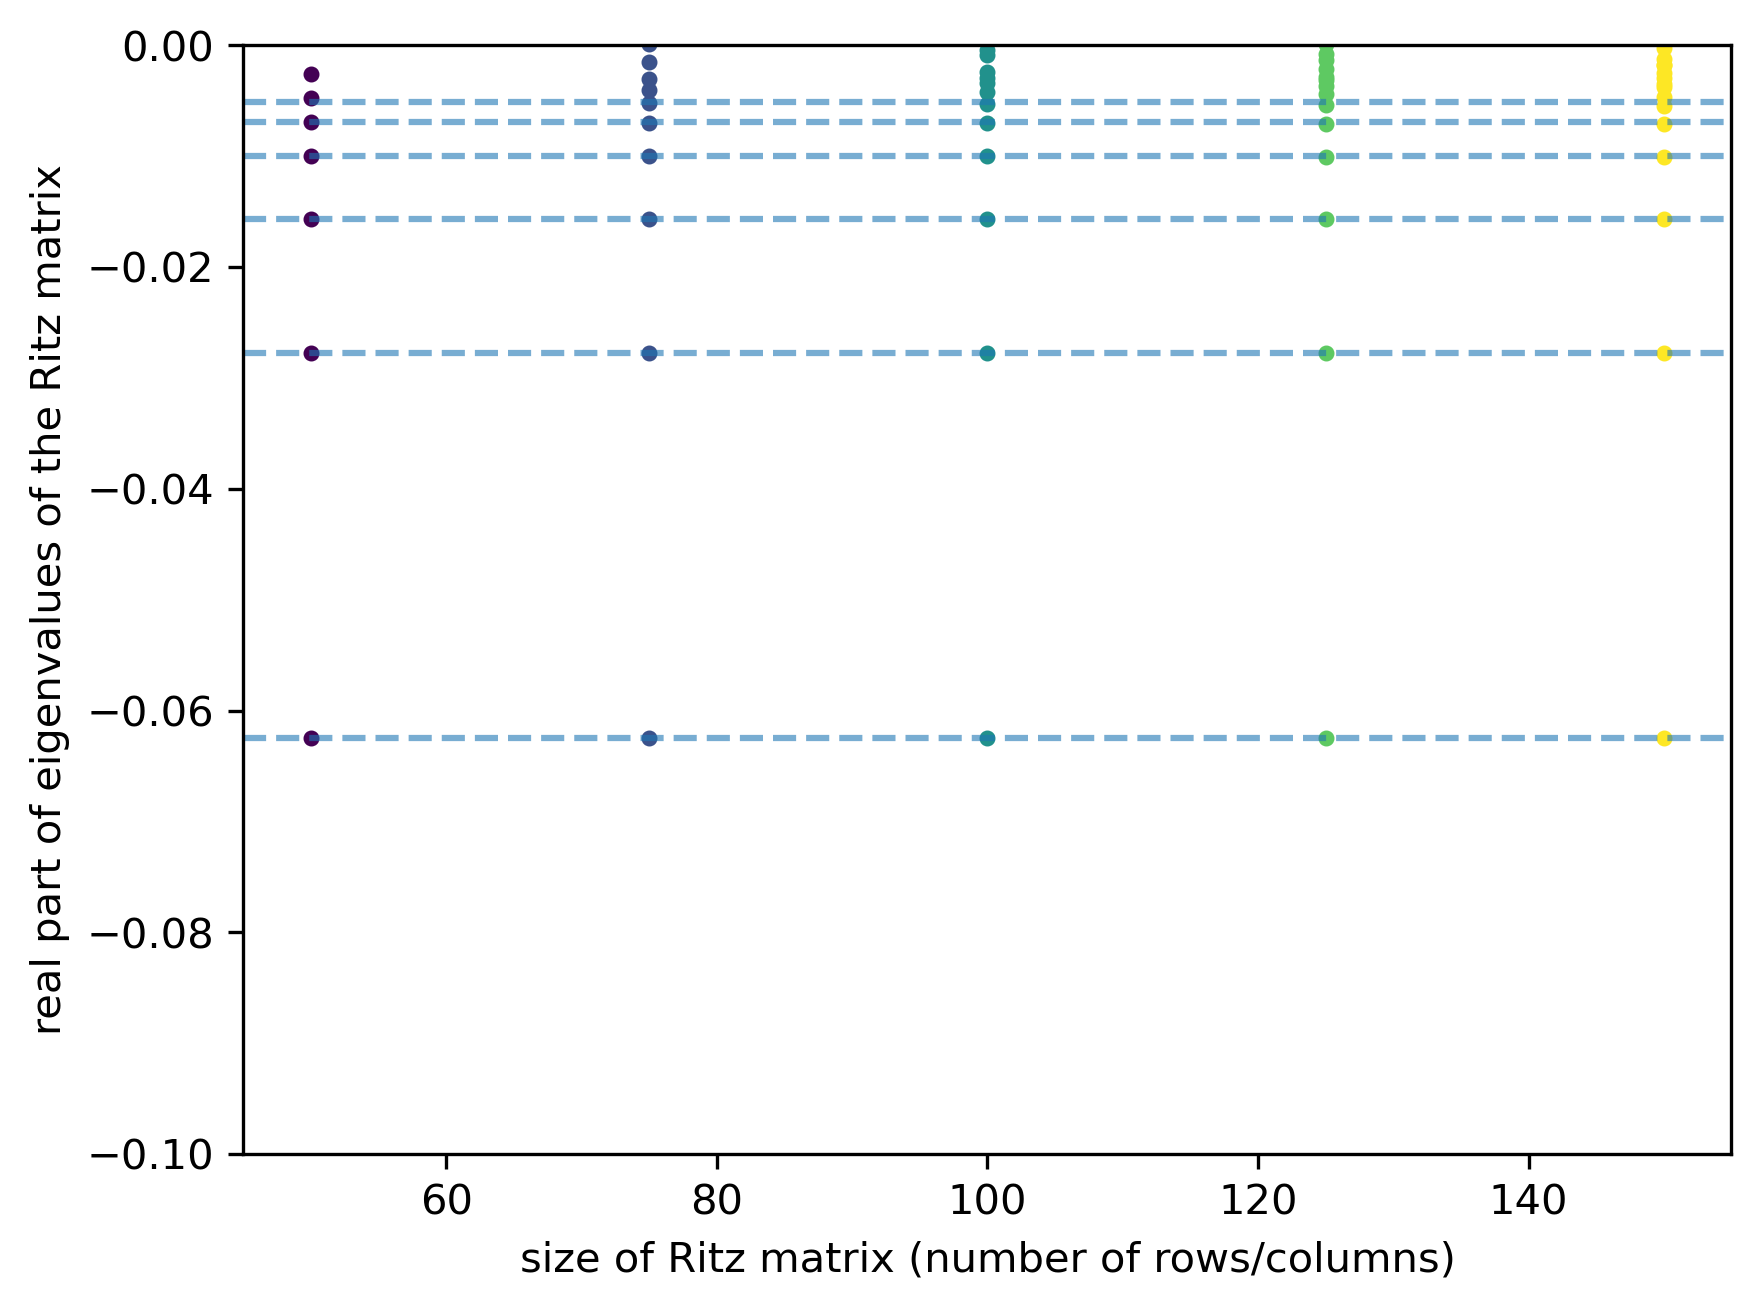
\includegraphics{hydrogen}
\caption{A Ritz-Galerkin approximation for the Schr\"odinger operator given above, cropped to ignore the positive spectrum (which is known to be the whole positive half-axis). The dotted lines correspond to where the first 6 eigenvalues should be according to the formula.
Note how as the size of the Ritz matrix increases, the higher eigenvalues (closer to the origin, as they are a sequence converging to 0) `fill in'.}\label{fig:schrodinger-ritz}
\end{figure}
\clearpage


Indeed, comparing this derivation to the earlier definitions of truncations, we can see that we are calculating the eigenvalues of truncations $T_n$ of the
operator $T$. The natural question which follows is to ask about the convergence of these methods as $n$ becomes large. The answer is that this
convergence is not perfect. The spectrum of the operator will be approximated, but in many cases there will also be a lot of other spurious values in the spectrum.
This brings us to our main subject; the study of these spurious eigenvalues, known as spectral pollution.

\subsection{Spectral pollution}

\begin{definition}{\textbf{(Spectral pollution)}}\index{spectrum!pollution of}
(Adapted from \parencite{davies1995spectral})
Let $(T_n)_{n \in \mathbb{N}}$ be an increasing sequence of truncations of an operator $T$. A value $\lambda \in \mathbb{C}$ is said to be a point of \textbf{spectral pollution} if there is a sequence $\lambda_n \in \Spec(T_n)$ such that $\lambda_n \rightarrow \lambda$ but $\lambda \notin \Spec(T)$.
\end{definition}

Points of spectral pollution are, intuitively, artefacts of the approximation which will never converge to a point in the actual spectrum. We will see that they exist, that they are relatively common, and that they \emph{get worse} as the approximation goes to higher iterations. Unless we already
know what the spectrum of the operator is, it can be incredibly hard for us to decide whether a point is actually in the spectrum or whether it is
spurious. In applications of spectral theory, this difference can be beyond a simple 'noisy data' nuisance - rather, a confounding problem.

\begin{example}
%TODO
\end{example}

We see in Figure \ref{fig:TODO} that this approximation does not work so well. It looks like it successfully covers the relevant parts of the spectrum,
but there are a lot of additional eigenvalues which do not exist!

There are, of course, other methods for approximating operator spectra, such as the popular finite difference or `shooting' methods \cite{suli2003introduction}, or specialised algebraic methods \cite{aceto2006numerical}, which are not subject to pollution. So why do we
care about truncation methods?
The motivation for studying Ritz-Galerkin methods is that they make \emph{almost no} assumptions about the operator itself or the location of its spectrum. 
If the spectral pollution for a sequence of truncations can be discarded, detected or otherwise dealt with, it would provide a unified and 
powerful approach to numerical spectral theory for almost any operator.
\end{document}